\documentclass{article}

% Language setting
% Replace `english' with e.g. `spanish' to change the document language
\usepackage[english]{babel}
\usepackage{listings}
\usepackage{xcolor}

\definecolor{codegreen}{rgb}{0,0.6,0}
\definecolor{codegray}{rgb}{0.5,0.5,0.5}
\definecolor{codepurple}{rgb}{0.8,0,0.2}
\definecolor{backcolour}{rgb}{.95,.95,1}

\lstdefinestyle{mystyle}{
    backgroundcolor=\color{backcolour},   
    commentstyle=\color{codegreen},
    keywordstyle=\color{blue},
    numberstyle=\tiny\color{codegray},
    stringstyle=\color{codepurple},
    basicstyle=\ttfamily\footnotesize,
    breakatwhitespace=false,         
    breaklines=true,                 
    captionpos=b,                    
    keepspaces=true,                 
    numbers=left,                    
    numbersep=5pt,                  
    showspaces=false,                
    showstringspaces=false,
    showtabs=false,                  
    tabsize=2
}

% Set page size and margins
% Replace `letterpaper' with `a4paper' for UK/EU standard size
\usepackage[letterpaper,top=2cm,bottom=2cm,left=3cm,right=3cm,marginparwidth=1.75cm]{geometry}

% Useful packages
\usepackage{amsmath}
\usepackage{graphicx}
\usepackage[colorlinks=true, allcolors=blue]{hyperref}

\title{Implementação 3 - Grafos }
\author{Daniel Salgado, Arthur Martinho }

\lstset{style=mystyle}

\begin{document}


\date{10/10/2024}
\maketitle



\section{Algoritmo de Djikstra em C++}

%código de djikstra

\begin{lstlisting}[language=c++ ,caption = Exemplo C++]
#include <iostream>
#include <vector>
#include <climits> // Para usar INT_MAX como infinito
#include <algorithm> // Para usar reverse

using namespace std;

struct Aresta {
    int destino, peso;
};

struct Vertice {
    int distancia = INT_MAX; // Distância inicial é infinito
    int antecessor = -1;     // Antecessor inicial é indefinido
    bool visitado = false;   // Indica se o vértice já foi visitado
};

// Função que mostra o caminho e a distância de origem até destino
void mostrarCaminho(int destino, int origem, const vector<Vertice>& vertices) {
    if (vertices[destino].distancia == INT_MAX) {
        cout << "Não há caminho de " << origem << " para " << destino << endl;
    } else {
        vector<int> caminho;
        for (int v = destino; v != -1; v = vertices[v].antecessor) {
            caminho.push_back(v);
        }
        reverse(caminho.begin(), caminho.end());

        cout << "Caminho de " << origem << " para " << destino << ": ";
        for (size_t i = 0; i < caminho.size(); i++) {
            cout << caminho[i];
            if (i < caminho.size() - 1) cout << " -> ";
        }
        cout << " | Distância: " << vertices[destino].distancia << endl;
    }
}

void dijkstra(int n, int origem, vector<vector<Aresta>>& grafo, vector<Vertice>& vertices) {
    
    vertices[origem].distancia = 0; // A distância do vértice de origem para ele mesmo é 0

    for (int k = 0; k < n; k++) {
        // Encontra o vértice não visitado com a menor distância
        int y1 = -1;
        for (int i = 0; i < n; i++) {
            if (!vertices[i].visitado && (y1 == -1 || vertices[i].distancia < vertices[y1].distancia)) {
                y1 = i;
            }
        }

        if (y1 == -1) {
            break; // Se não houver mais vértices para visitar, termina
        }

        vertices[y1].visitado = true; // Marca o vértice como visitado

        // Atualiza as distâncias dos vizinhos de y1
        for (const Aresta& vizinho : grafo[y1]) {
            if (!vertices[vizinho.destino].visitado) {
                int novaDistancia = vertices[y1].distancia + vizinho.peso;
                if (novaDistancia < vertices[vizinho.destino].distancia) {
                    vertices[vizinho.destino].distancia = novaDistancia;
                    vertices[vizinho.destino].antecessor = y1; // Atualiza o antecessor
                }
            }
        }
    }


    // Mostra as distâncias e os caminhos para todos os vértices
    for (int i = 0; i < n; i++) {
        mostrarCaminho(i, origem,vertices);
    }
}

int main() {
    int n = 5; // Número de vértices

    vector<Vertice> vertices(n); // Vetor que armazena informações de cada vértice

    vector<vector<Aresta>> grafo(n); // o grafo é um vetor de inteiros(vertices), onde cada vertice possui um vetor de arestas

    // Adiciona as arestas ao grafo (Exemplo de grafo)
    grafo[0].push_back({1, 4});
    grafo[0].push_back({2, 3});
    grafo[1].push_back({2, 5});
    grafo[1].push_back({3, 2});
    grafo[2].push_back({4, 3});
    grafo[2].push_back({3, 1});
    grafo[3].push_back({4, 4});

    int origem = 0; // Vértice inicial (origem)

    dijkstra(n, origem, grafo, vertices);

    return 0;
}

\end{lstlisting}
\subsection{Como Funciona}

\paragraph{Função mostrarCaminho: mostra o caminho e a distância de origem até destino. A função começa verificando se existe um caminho até o destino, se houver um caminho válido, a função percorre os antecessores dos vértices, começando pelo destino, até chegar na origem, construindo um vetor chamado caminho que contém os vértices nessa ordem. Por fim, a função exibe o caminho completo da origem até o destino, separando cada vértice com ->, e, em seguida, imprime a distância total do caminho.}

\paragraph{Função djikstra: define a distância do vértice de origem como 0, pois a distância dele para ele mesmo é zero. Na iteração principal, para cada vértice, busca o vértice não visitado que tenha a menor distância atual. Se não houver mais vértices para visitar (todos foram processados ou são inacessíveis), interrompe a execução. Cada iteração marcará o vértice com a menor distância como visitado e para cada vizinho desse vértice, calcula a nova distância potencial. Se essa nova distância for menor do que a distância armazenada atualmente no vizinho, atualiza a distância e define o vértice antecessor. Após processar todos os vértices, a função chama a função mostrarCaminho para exibir os caminhos e as distâncias mínimas de todos os vértices a partir da origem.}

\paragraph{Função main: Informa o número de vértices e cria um vetor para armazenar os vértices e arestas. A função main adiciona arestas ao grafo e chama a função de djikstra, passando como parâmetros o número de vértices, o vértice de origem, o vetor de inteiro vértices e o vetor que armazena as informações de cada vértice.}

\subsection{ Teste do Código }

\begin{figure}[h]
    \centering
    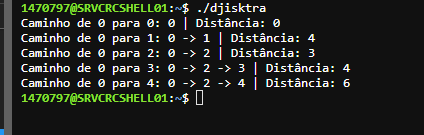
\includegraphics[width=1\textwidth]{imgs/djikstra.PNG}
    \caption{Teste Djikstra}
    \label{fig:corr}
\end{figure}
\

\section{Algoritmo MinMax em C++}
%código de MinMax
\begin{lstlisting}[language=c++ ,caption = Exemplo C++]
#include <iostream>
#include <vector>
#include <climits> // Para usar INT_MAX como infinito
#include <algorithm> // Para usar reverse
#include <queue> // Para usar fila de prioridade

using namespace std;

struct Aresta {
    int destino, peso;
};

struct Vertice {
    int dist = INT_MAX; // Inicialmente a menor distância é infinito
    int antecessor = -1; // Antecessor inicial é indefinido
};

void mostrarCaminho(int destino, int origem, const vector<Vertice>& vertices) {
    if (vertices[destino].dist == INT_MAX) {
        cout << "Não há caminho de " << origem << " para " << destino << endl;
    } else {
        vector<int> caminho;
        for (int v = destino; v != -1; v = vertices[v].antecessor) {
            caminho.push_back(v);
        }
        reverse(caminho.begin(), caminho.end());

        cout << "Caminho de " << origem << " para " << destino << ": ";
        for (size_t i = 0; i < caminho.size(); i++) {
            cout << caminho[i];
            if (i < caminho.size() - 1) cout << " -> ";
        }
        cout << " | Peso da maior aresta: " << vertices[destino].dist << endl;
    }
}

void minMax(int n, int origem, vector<vector<Aresta>>& grafo, vector<Vertice>& vertices) {
    // Inicializa a distância do vértice de origem
    vertices[origem].dist = 0; // A distância inicial é 0

    // Usamos uma fila de prioridade para selecionar a aresta com o menor peso máximo
    priority_queue<pair<int, int>, vector<pair<int, int>>, greater<pair<int, int>>> pq; // par (peso, vértice)
    pq.push({0, origem}); // Começamos com a origem

    while (!pq.empty()) {
        auto [peso, u] = pq.top(); // Pega o menor peso máximo
        pq.pop();

        // Se a distância do vértice atual é menor que a já registrada, ignoramos
        if (vertices[u].dist < peso) continue;

        // Atualiza as distâncias acumuladas dos vizinhos de u
        for (const Aresta& vizinho : grafo[u]) {
            int novaDist = max(vertices[u].dist, vizinho.peso); // O peso máximo do caminho
            // Se encontramos um caminho com um peso máximo menor
            if (novaDist < vertices[vizinho.destino].dist) {
                vertices[vizinho.destino].dist = novaDist;
                vertices[vizinho.destino].antecessor = u; // Atualiza o antecessor
                pq.push({novaDist, vizinho.destino}); // Adiciona à fila de prioridade
            }
        }
    }

    // Mostra os caminhos para todos os vértices
    for (int i = 0; i < n; i++) {
        if (i == origem)
            continue;
        mostrarCaminho(i, origem, vertices);
    }
}

int main() {
    int n = 5; // Número de vértices

    vector<Vertice> vertices(n); // Vetor que armazena informações de cada vértice

    vector<vector<Aresta>> grafo(n); // o grafo é um vetor de inteiros (vértices), onde cada vértice possui um vetor de arestas

    // Adiciona as arestas ao grafo (Exemplo de grafo)
    grafo[0].push_back({1, 4});
    grafo[0].push_back({2, 3});
    grafo[1].push_back({2, 5});
    grafo[1].push_back({3, 2});
    grafo[2].push_back({4, 3});
    grafo[2].push_back({3, 1});
    grafo[3].push_back({4, 4});

    int origem = 0; // Vértice inicial (origem)

    minMax(n, origem, grafo, vertices);

    return 0;
}

\end{lstlisting}
\subsection{Como Funciona}

\paragraph{Função mostrarCaminho: mostra o caminho e a distância de origem até destino. A função começa verificando se existe um caminho até o destino, se houver um caminho válido, a função percorre os antecessores dos vértices, começando pelo destino, até chegar na origem, construindo um vetor chamado caminho que contém os vértices nessa ordem. Por fim, a função exibe o caminho completo da origem até o destino, separando cada vértice com ->, e, em seguida, imprime a distância total do caminho.}

\paragraph{A função minMax implementa um algoritmo para encontrar o caminho que minimiza o peso máximo das arestas em um grafo, ou seja, busca maximizar a largura de banda do caminho de origem até todos os outros vértices.}

\paragraph{Função minMax: define a distância do vértice de origem como 0, pois a distância dele para ele mesmo é zero. Em seguida, utiliza-se uma fila de prioridade (priority-queue) configurada para retornar o menor peso máximo, iniciando com a origem e um peso de 0. Durante o processamento, enquanto a fila não estiver vazia, o algoritmo seleciona e remove o vértice com o menor peso máximo; se a distância registrada desse vértice for menor do que o peso, ele é ignorado. Para cada vizinho, calcula-se a nova distância como o máximo entre a distância acumulada atual e o peso da aresta, e, se essa nova distância for menor do que a registrada para o vizinho, a distância é atualizada e o antecessor é ajustado. O vizinho é então adicionado à fila para processamento posterior. Ao final, a função exibe os caminhos e as distâncias minimizadas máximas da origem para todos os outros vértices, utilizando mostrarCaminho. Em relação às variáveis, utilizamos vertices[u].dist para armazenar o peso máximo do caminho minimizado, vertices[u].antecessor para indicar o vértice anterior, grafo[u] que representa os vizinhos conectados e a fila de prioridade que assegura a minimização do peso máximo.}

\paragraph{Função main: Informa o número de vértices e cria um vetor para armazenar os vértices e arestas. A função main adiciona arestas ao grafo e chama a função de minMax, passando como parâmetros o número de vértices, o vértice de origem, o vetor de inteiro vértices e o vetor que armazena as informações de cada vértice.}

\subsection{ Teste do Código }

\begin{figure}[h]
    \centering
    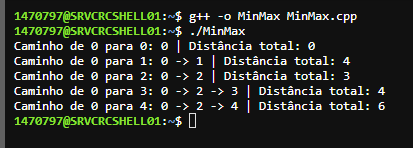
\includegraphics[width=1\textwidth]{imgs/MinMax.PNG}
    \caption{Teste MinMax}
    \label{fig:corr}
\end{figure}
\

\section{Algoritmo MaxMin em C++}
%código de MaxMin
\begin{lstlisting}[language=c++ ,caption = Exemplo C++]
#include <iostream>
#include <vector>
#include <climits> // Para usar INT_MAX como infinito
#include <algorithm> // Para usar reverse
#include <queue> // Para usar fila de prioridade

using namespace std;

struct Aresta {
    int destino, peso;
};

struct Vertice {
    int dist = INT_MIN; // Inicialmente a menor distância é menos infinito
    int antecessor = -1; // Antecessor inicial é indefinido
};

void mostrarCaminho(int destino, int origem, const vector<Vertice>& vertices) {
    if (vertices[destino].dist == INT_MIN) {
        cout << "Não há caminho de " << origem << " para " << destino << endl;
    } else {
        vector<int> caminho;
        for (int v = destino; v != -1; v = vertices[v].antecessor) {
            caminho.push_back(v);
        }
        reverse(caminho.begin(), caminho.end());

        cout << "Caminho de " << origem << " para " << destino << ": ";
        for (size_t i = 0; i < caminho.size(); i++) {
            cout << caminho[i];
            if (i < caminho.size() - 1) cout << " -> ";
        }
        cout << " | Peso da menor aresta: " << vertices[destino].dist << endl;
    }
}

void maxMin(int n, int origem, vector<vector<Aresta>>& grafo, vector<Vertice>& vertices) {
    // Inicializa a distância do vértice de origem
    vertices[origem].dist = INT_MAX; // Máximo inicialmente

    // Usamos uma fila de prioridade para selecionar a aresta com o maior peso
    priority_queue<pair<int, int>> pq; // par (peso, vértice)
    pq.push({INT_MAX, origem}); // Começamos com a origem

    while (!pq.empty()) {
        auto [peso, u] = pq.top(); // Pega o maior peso
        pq.pop();

        // Se a distância do vértice atual é menor que a já registrada, ignoramos
        if (vertices[u].dist > peso) continue;

        // Atualiza as distâncias acumuladas dos vizinhos de u
        for (const Aresta& vizinho : grafo[u]) {
            int novaDist = min(vertices[u].dist, vizinho.peso);
            // Se encontramos um caminho com um peso maior
            if (novaDist > vertices[vizinho.destino].dist) {
                vertices[vizinho.destino].dist = novaDist;
                vertices[vizinho.destino].antecessor = u; // Atualiza o antecessor
                pq.push({novaDist, vizinho.destino}); // Adiciona à fila de prioridade
            }
        }
    }

    // Mostra os caminhos para todos os vértices
    for (int i = 0; i < n; i++) {
        if(i == origem)
            continue;
        mostrarCaminho(i, origem, vertices);
    }
}

int main() {
    int n = 5; // Número de vértices

    vector<Vertice> vertices(n); // Vetor que armazena informações de cada vértice

    vector<vector<Aresta>> grafo(n); // o grafo é um vetor de inteiros (vértices), onde cada vértice possui um vetor de arestas

    // Adiciona as arestas ao grafo (Exemplo de grafo)
    grafo[0].push_back({1, 4});
    grafo[0].push_back({2, 3});
    grafo[1].push_back({2, 5});
    grafo[1].push_back({3, 2});
    grafo[2].push_back({4, 3});
    grafo[2].push_back({3, 1});
    grafo[3].push_back({4, 4});

    int origem = 0; // Vértice inicial (origem)

    maxMin(n, origem, grafo, vertices);

    return 0;
}

\end{lstlisting}
\subsection{Como Funciona}

\paragraph{Função mostrarCaminho: mostra o caminho e a distância de origem até destino. A função começa verificando se existe um caminho até o destino, se houver um caminho válido, a função percorre os antecessores dos vértices, começando pelo destino, até chegar na origem, construindo um vetor chamado caminho que contém os vértices nessa ordem. Por fim, a função exibe o caminho completo da origem até o destino, separando cada vértice com ->, e, em seguida, imprime a distância total do caminho.}

\paragraph{A função maxMin é uma variação de um algoritmo de caminhos mínimos que, em vez de buscar o caminho de menor custo, encontra o caminho que maximiza o menor peso ao longo das arestas do grafo. O objetivo é encontrar um caminho em que o menor peso de todas as arestas no caminho seja o maior possível.}

\paragraph{Função maxMin: define a distância do vértice de origem como 0, pois a distância dele para ele mesmo é zero. Em seguida, utiliza-se uma fila de prioridade (priority-queue) para selecionar a aresta com o maior peso disponível, inicializando-a com a origem e o valor INT-MAX. Enquanto a fila não estiver vazia, o algoritmo processa o vértice com a maior distância acumulada, removendo-o da fila. Se a distância do vértice atual for menor que a registrada, ele é ignorado. Para cada vizinho do vértice atual, calcula-se uma nova distância acumulada como o menor valor entre a distância atual e o peso da aresta para o vizinho. Se esse valor for maior que a distância registrada do vizinho, ela é atualizada, e o antecessor é definido como o vértice atual. O vizinho é então adicionado à fila para processamento. Após analisar todos os vértices, a função exibe os caminhos e as distâncias máximas mínimas da origem para os outros vértices usando mostrarCaminho. Em relação às variáveis, utilizamos vertices[u].dist para armazenar a maior distância mínima, vertices[u].antecessor para indicar o vértice anterior no caminho, grafo[u] para listar os vizinhos, e priority-queue para garantir o processamento dos vértices que maximizam o menor peso possível.}

\paragraph{Função main: Informa o número de vértices e cria um vetor para armazenar os vértices e arestas. A função main adiciona arestas ao grafo e chama a função de maxMin, passando como parâmetros o número de vértices, o vértice de origem, o vetor de inteiro vértices e o vetor que armazena as informações de cada vértice.}

\subsection{ Teste do Código }

\begin{figure}[h]
    \centering
    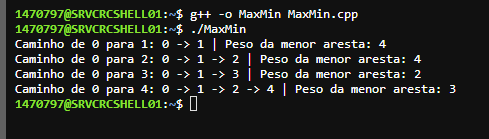
\includegraphics[width=1\textwidth]{imgs/MaxMin.PNG}
    \caption{Teste MaxMin}
    \label{fig:corr}
\end{figure}
\


\newpage

\newpage

\end{document}